\begin{figure}[ht]
\centering
\resizebox{\textwidth}{!}{
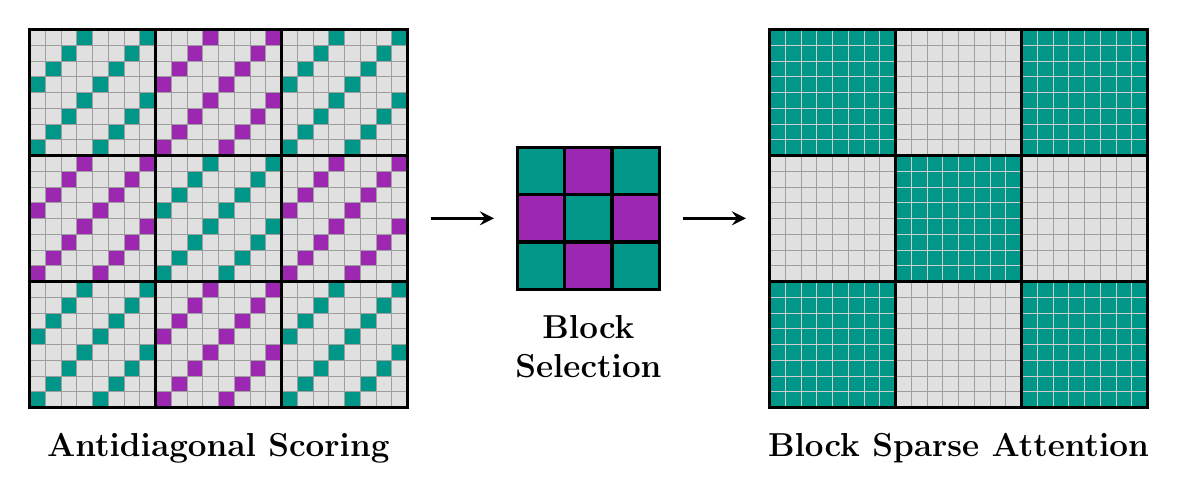
\begin{tikzpicture}[>=stealth, thick]

  % Colors
  \definecolor{selcolor}{HTML}{009688} % Teal
  \definecolor{unselcolor}{HTML}{9C27B0} % Purple
  \definecolor{bglight}{HTML}{E0E0E0}
  \definecolor{gridcolor}{HTML}{9E9E9E}

  \def\cell{0.2} % cell size for left and right
  \def\bcell{1.6} % big cell size = 8 * 0.2

  % PART 1: Antidiagonal Scoring
  \begin{scope}[shift={(0,0)}]
    % Draw background and small grid
    \fill[bglight] (0,0) rectangle (3*\bcell, -3*\bcell);
    \draw[gridcolor, very thin, step=\cell] (0,0) grid (3*\bcell, -3*\bcell);
    
    % Draw antidiagonals
    \foreach \br in {0,1,2} {
      \foreach \bc in {0,1,2} {
        % Determine if block is selected: X pattern => br == bc or br+bc == 2
        \pgfmathtruncatemacro{\issel}{(\br==\bc) || (\br+\bc==2)}
        \ifnum\issel=1
          \colorlet{dcolor}{selcolor}
        \else
          \colorlet{dcolor}{unselcolor}
        \fi
        
        \foreach \r in {0,...,7} {
          \foreach \c in {0,...,7} {
            % Antidiagonal of each S x S sub-block (S=4): the cells where
            % the local row and column index sum to S-1, i.e. r+c == 3 (mod 4).
            % Drawn over the full block without the causal mask for clarity.
            \pgfmathtruncatemacro{\isdiag}{mod(\r+\c,4)==3}
            \ifnum\isdiag=1
              \fill[dcolor] ({\bc*\bcell + \c*\cell}, {-\br*\bcell - \r*\cell}) rectangle ++(\cell, -\cell);
              \draw[gridcolor, very thin] ({\bc*\bcell + \c*\cell}, {-\br*\bcell - \r*\cell}) rectangle ++(\cell, -\cell);
            \fi
          }
        }
      }
    }
    % Draw thick big block borders
    \draw[very thick, step=\bcell] (0,0) grid (3*\bcell, -3*\bcell);
    \draw[very thick] (0,0) rectangle (3*\bcell, -3*\bcell);
    \node[below, font=\large\bfseries] at (1.5*\bcell, -3*\bcell - 0.2) {Antidiagonal Scoring};
  \end{scope}

  % Arrow 1
  \draw[->, very thick] (3*\bcell + 0.3, -1.5*\bcell) -- ++(0.8, 0);

  % PART 2: Block Selection
  % The middle grid is 3x3, let's make it smaller, e.g. cell size 0.6
  \def\mcell{0.6}
  \begin{scope}[shift={(3*\bcell + 1.4, -1.5*\bcell + 1.5*\mcell)}]
    \foreach \br in {0,1,2} {
      \foreach \bc in {0,1,2} {
        \pgfmathtruncatemacro{\issel}{(\br==\bc) || (\br+\bc==2)}
        \ifnum\issel=1
          \fill[selcolor] (\bc*\mcell, -\br*\mcell) rectangle ++(\mcell, -\mcell);
        \else
          \fill[unselcolor] (\bc*\mcell, -\br*\mcell) rectangle ++(\mcell, -\mcell);
        \fi
        \draw[very thick] (\bc*\mcell, -\br*\mcell) rectangle ++(\mcell, -\mcell);
      }
    }
    \draw[very thick] (0,0) rectangle (3*\mcell, -3*\mcell);
    \node[below, align=center, font=\large\bfseries] at (1.5*\mcell, -3*\mcell - 0.2) {Block\\Selection};
  \end{scope}

  % Arrow 2
  \draw[->, very thick] (3*\bcell + 1.4 + 3*\mcell + 0.3, -1.5*\bcell) -- ++(0.8, 0);

  % PART 3: Block Sparse Attention
  \begin{scope}[shift={(3*\bcell + 1.4 + 3*\mcell + 1.4, 0)}]
    \fill[bglight] (0,0) rectangle (3*\bcell, -3*\bcell);
    \draw[gridcolor, very thin, step=\cell] (0,0) grid (3*\bcell, -3*\bcell);
    
    \foreach \br in {0,1,2} {
      \foreach \bc in {0,1,2} {
        \pgfmathtruncatemacro{\issel}{(\br==\bc) || (\br+\bc==2)}
        \ifnum\issel=1
          \fill[selcolor] (\bc*\bcell, -\br*\bcell) rectangle ++(\bcell, -\bcell);
          % We can re-draw the small grid over it if we want it to look like the original
          \draw[gridcolor!50!white, very thin, step=\cell, shift={(\bc*\bcell, -\br*\bcell)}] (0,0) grid (\bcell, -\bcell);
        \fi
      }
    }
    
    \draw[very thick, step=\bcell] (0,0) grid (3*\bcell, -3*\bcell);
    \draw[very thick] (0,0) rectangle (3*\bcell, -3*\bcell);
    \node[below, font=\large\bfseries] at (1.5*\bcell, -3*\bcell - 0.2) {Block Sparse Attention};
  \end{scope}

\end{tikzpicture}
}
\caption{XAttention three-stage process: Antidiagonal scoring samples $S{\times}S$ antidiagonals to estimate block importance. Block selection picks the top-scoring blocks. Block sparse attention computes the full attention only for selected blocks. For brevity we draw the antidiagonals over the full block and do not show the causal mask.}
\label{fig:xattention_3part}
\end{figure}
